\documentclass[10pt,a4paper]{article}
\usepackage[margin=23mm]{geometry}
\usepackage{nature_reading}
\usepackage{longtable}
% Generated from pinned audit evidence.
\newcommand{\TrainSeconds}{361.6}
\newcommand{\TrainMemory}{0.543}
\newcommand{\FirstIdentity}{1.17}
\newcommand{\FirstShuffled}{1.17}
\newcommand{\FirstZero}{0.00}
\newcommand{\BlockIdentity}{0.586}
\newcommand{\BlockGain}{0.098}
\newcommand{\BlockLow}{0.000}
\newcommand{\BlockHigh}{0.307}
\newcommand{\BlockFone}{0.320}
\newcommand{\RunDecision}{reject}

% Generated from the pinned V54 audit; no fitted presentation values.
\newcommand{\DensitySeconds}{207.8}
\newcommand{\DensityMemory}{0.400}
\newcommand{\DensityNll}{15.219}
\newcommand{\DensityShuffledNll}{15.254}
\newcommand{\DensityAdvantage}{0.0355}
\newcommand{\DensityLow}{-0.1014}
\newcommand{\DensityHigh}{0.1693}
\newcommand{\DensityIdentity}{1.562}
\newcommand{\DensityFone}{0.350}
\newcommand{\DensityCopyFone}{0.99949}
\newcommand{\DensityDecision}{reject}

% Generated from the locked V55 matched audit.
\newcommand{\JointNll}{7.026}
\newcommand{\ControlNll}{7.579}
\newcommand{\JointNllGain}{0.553}
\newcommand{\JointNllLow}{0.450}
\newcommand{\JointNllHigh}{0.665}
\newcommand{\JointTime}{342.4}
\newcommand{\ControlTime}{218.0}
\newcommand{\JointMemory}{0.648}
\newcommand{\ControlMemory}{0.400}
\newcommand{\JointSampleFone}{0.362}
\newcommand{\JointPrefixGain}{0.185}
\newcommand{\JointDecision}{reject}

% Generated from unchanged V56 report.
\newcommand{\BeamAccuracy}{11.621}
\newcommand{\BeamShuffled}{9.863}
\newcommand{\GreedyAccuracy}{8.252}
\newcommand{\BeamGain}{3.369}
\newcommand{\BeamGainLow}{2.351}
\newcommand{\BeamGainHigh}{4.412}
\newcommand{\BeamHistoryGain}{1.758}
\newcommand{\BeamHistoryLow}{0.966}
\newcommand{\BeamHistoryHigh}{2.552}
\newcommand{\BeamRepeat}{25.446}
\newcommand{\TargetRepeat}{0.112}
\newcommand{\BeamSeconds}{269.3}
\newcommand{\BeamMemory}{0.154}
\newcommand{\BeamDecision}{reject\_decoder}

% Generated from the completed V57 audit.
\newcommand{\QaExact}{3.906}
\newcommand{\QaFone}{15.718}
\newcommand{\QaBlankExact}{0.391}
\newcommand{\QaBlankFone}{5.553}
\newcommand{\QaControlExact}{0.000}
\newcommand{\QaControlFone}{6.582}
\newcommand{\QaQuestionGain}{10.165}
\newcommand{\QaQuestionLow}{7.043}
\newcommand{\QaQuestionHigh}{13.371}
\newcommand{\QaPairExact}{0.254}
\newcommand{\QaMotor}{100.000}
\newcommand{\QaSeconds}{278.572}
\newcommand{\QaMemory}{1.053}
\newcommand{\QaControlSeconds}{269.126}
\newcommand{\QaControlMemory}{1.049}
\newcommand{\QaDecision}{reject\_reading\_model}

\begin{document}
\renewcommand{\thefigure}{S\arabic{figure}}
{\sffamily\bfseries\Large Supplementary Information\par}
\medskip\noindent\textbf{Learning conditional language in continuous image space}\par
\medskip\noindent Imagized Language Model Project

\section*{Supplementary Note 1: experimental question and scope}
The target is an independent visual language model whose runtime consumes
writing images and generates writing images. Encoded text and local language
models may prepare data offline. They cannot supply the answer during model
inference. The present experiment isolates canonical Chinese continuation as
one prerequisite. It does not cover the complete instruction-following or
historical-script objective.

The repository retains the earlier 96-page research record in its legacy
image-native publication folder. That record documents prior
experiments without treating every rejected architecture as a contribution to
the compact article. This supplement specifies the directly conditional
block test, the subsequent exact-raster density and the distinction between
ranking and generation.

\section*{Supplementary Note 2: conditional uncertainty}
Let $H$ denote a visible history and $X$ the next writing image. Under squared
pixel loss, the optimum $f^*(H)=\mathbb{E}[X\mid H]$ can mix valid glyphs.
Under independent Bernoulli loss, each marginal equals
$\Pr(X_p=1\mid H)$, which likewise does not specify joint stroke identity.
An image distribution is consequently required for stochastic writing.

Selection and sampling have different expected identity accuracy. If a
model exactly recovers the true next-form distribution $p(x\mid H)$,
deterministic top-1 identity has conditional accuracy
$\max_x p(x\mid H)$. Independently sampling one future and comparing it to
one observed continuation has expected accuracy $\sum_x p(x\mid H)^2$.
Neither quantity is a general measure of semantic correctness. Thus the
reader's 19.97\% top-1 cannot be used as the expected accuracy of a correct
stochastic writer. Paired context controls, sampled probabilities, direct
readability and meaningful longer continuations are needed together.

\section*{Supplementary Note 3: raster transform and gradients}
For signed ink image $S=2X-1$ and a $32\times32$ orthonormal basis $B$, the
visual coordinate is
\begin{equation}
\phi(S)=\frac{\operatorname{vec}(BSB^{\mathsf T})}
{\|\operatorname{vec}(BSB^{\mathsf T})\|_2}.
\end{equation}
For binary observed images this matches the reader's field. For soft predicted
images it must be computed directly on $S$. Applying the reader's input
threshold inside this training objective would cut all pixel gradients.
The pretraining inspection found and corrected that defect. A regression test
confirms a finite, nonzero gradient from the field cosine alone to the predicted
pixels and equality with the reader transform on binary inputs.

The transform is a full spatial coordinate, not a learned visual vocabulary.
Its background contribution also limits its interpretation as a perceptual
identity metric. A high cosine can accompany an incorrect glyph.

\section*{Supplementary Note 4: directly conditional architecture}
The frozen reader has 16,277,249 parameters. Its final 384-dimensional hidden
state and 1,024-dimensional anchor form a continuous condition. A 5,899,970-
parameter U-Net receives a complete $32\times128$ future strip. Three spatial
scales have 64, 128 and 256 channels. Each residual scale receives the projected
condition and a sinusoidal time embedding. Additional input channels carry the
first-cell predicted plan, a horizontal coordinate and the cell noise levels.

At the bottleneck, four pooled cell vectors enter four-head attention and a
512-wide MLP. A zero-initialized scalar gates the spatial mixer residual.
The output channel predicts velocity over four visible cells. The total
runtime contains 22,177,219 parameters. The prior checkpoint only initializes
matching U-Net weights. An epsilon predictor is not thereby a qualified
velocity predictor, so all copied layers are fine-tuned under the new loss.

\section*{Supplementary Note 5: data and optimization}
The corpus manifest SHA-256 is
\begin{quote}\small\ttfamily
76048753b52735d14c98f0d9e4eb8d751401fe8810e82eaaaebff517f6866c03.
\end{quote}
Source identifiers define deterministic splits before rendering. Original and
OpenCC-simplified views inherit the same split. Data generation samples
65-cell segments with a saved dataset seed. Only the first 64 cells are used
in this test. A training example has 60 context and four target cells. A
symbolic character identifier is never an input or target to a model method.

On odd updates, the four future positions receive one level from each of
0--24, 25--59, 60--89 and 90--99 under a random permutation. On even updates,
one uniformly sampled level from 0--99 applies to all four future cells.
The latter pretraining amendment supplies synchronous noise patterns like
those encountered during sampling. It was frozen before optimization.

Ten percent of rows drop the condition. All-dropped batches have zero order
loss. The foreground loss weights pixels by $1+2X$. The complete objective is
\begin{align}
L={}&L_v+0.10L_{fg}+0.10L_{dice}+0.10L_{field}\nonumber\\
&+0.10L_{repr}+0.25L_{order},\\
L_{order}={}&\mathbb{E}_{t\geq60}\operatorname{softplus}
\left[0.02-(c_{ordered}-c_{shuffled})\right].
\end{align}
Only rows with an available condition enter the order loss. The reader remains
frozen. Noise, drop masks and data offsets derive from saved RNG states.
The run uses seed 20265310, dataset seed 20265311, AdamW with
$\beta=(0.9,0.95)$, weight decay 0.01, gradient norm clip 1, EMA decay 0.999,
batch eight and 8,000 updates. The full run consumes 64,000 context segments
and 256,000 supervised future cells. These are sampled segments rather than
64,000 independent source records.

\section*{Supplementary Note 6: locked audit and uncertainty}
The audit seed is 20265320. It uses 512 fixed development windows for
denoising, 256 for direct generation and 64 for two-block visible feedback.
The first 60 cells form the context and the remaining four context-window
cells form the first target block. The four subsequent continuation cells
form the second block. Denoising probes use levels 75 and 95, with identical
noise under all conditions. Prefix shuffling preserves the final four visible
cells. The zero condition removes all reader state and plan channels.

The 1,024-image bank is rendered after every denoising and generation call.
Every primary output is the first sample. Nearest-bank identity is evaluator
metadata, not an image replacement or glyph selected by the model. Per-position
coverage records how many true targets appear in the bank. All out-of-bank
targets receive zero exact-identity credit. The rendered output remains the
actual model image even when a bank identity is assigned.

Bootstrap uncertainty resamples source identifiers, retaining all correlated
windows from a record together, with 2,000 resamples. Paired differences keep
the same starting noise. The intervals do not include training-seed variation.
There is one primary trained seed and no sealed generalization result.

\section*{Supplementary Table 1: direct visual block audit}
\begin{center}\begin{tabular}{lrrrr}\toprule
Condition & First identity (\%) & Block identity (\%) & Pixel F1 & Isolated ink \\
\midrule
Ordered & 1.172 & 0.586 & 0.3198 & 0.0050 \\
Shuffled & 1.172 & 0.488 & 0.3176 & 0.0053 \\
Zero condition & 0.000 & 0.195 & 0.3018 & 0.0053 \\
\bottomrule\end{tabular}\end{center}
All 256 prefixes contribute one four-cell sample. Target coverage in the Han bank is 60.94, 58.98, 64.45 and 68.36\% by position. No out-of-bank target receives identity credit.


\section*{Supplementary Note 7: numerical and compute receipts}
Training takes \TrainSeconds\ seconds and peaks at \TrainMemory\ GiB of
allocated CUDA memory on GPU 0, an RTX 4090 D. These figures describe the
bounded experiment. They exclude prior foundation training, data preparation,
idle GPU memory, operating-system memory and evaluation. They are not an
estimate of the cost of a broadly capable language model. The independent
reader and prior training costs remain in their original run reports.

The continuous versus interrupted four-step smoke check compares every
denoiser and EMA tensor and the saved training generator. All match exactly.
Production checkpoints save optimizer groups, CPU/CUDA/Python/NumPy RNGs and
the deterministic data offset. Foundation, data, source and protocol hashes
are checked before scoring. No other project's GPU service is part of this run.

\section*{Supplementary Note 8: limitations and next evidence}
The post-result motor diagnostic uses the first 64 fixed prefixes and paired
noise. Replacing the first plan with the exact target raster gives F1 0.4586.
Replacing both plan and visual anchor gives F1 0.4594 and identity 5/64,
compared with F1 0.3775 and identity 1/64 for the predicted condition. An exact
inverse-transform control has F1 1.0. Only 60.94\% of these targets occur in
the Han identity bank, so its 60.94\% identity is the available ceiling for
perfect copies. The target-supplied test was designed after the locked audit
and does not change its decision. It isolates a remaining motor limitation.

Reliable autonomous continuation, calibrated conditional sequence likelihood,
held-out short answers, font transfer, independent seed replication and
capability-matched text baselines remain outstanding. No selected gallery can
substitute for these tests. Future teacher-generated exercises must retain
source provenance and separate prompt/answer splits. A deployed teacher or
an image-bank lookup would change the model contract.

The older guided model's terminal-signal observation is a mathematical limit,
not a proven failure explanation. Correct conditional diffusion also starts
from a context-independent noise law. Direct interventions on trained
conditional scores and matched initialization are needed to distinguish weak
condition learning from a defective sampling trajectory.

\section*{Supplementary Note 9: normalized raster density}
The exact-density model (V54) freezes the same 16,277,249-parameter reader.
A row transformer has width 192, four layers, six heads, MLP ratio three and
zero dropout. Its inputs are shifted earlier rows, a projection of the aligned
32-pixel plan row, spatial row positions and a projected continuous condition
(hidden384 plus field1024). A MADE with two 256-wide SiLU layers masks pixels
within each row. Its output mask is strict: pixel $c$ cannot see pixel $c$ or
any later pixel. Earlier rows may be observed in full. Gradients with respect
to forbidden pixels vanish even with nonzero randomized output weights.
Enumeration of all 16 four-bit outcomes gives total probability one.

The inverse reader field, scaled by 32 and clipped to $[-2,2]$, supplies an
aligned logit at scale six. Residual output weights start at zero. Thus a
supplied binary image has greedy reconstruction exactly equal to itself at
initialization. This copy path does not learn language and is not a lookup
bank. It applies to arbitrary supplied binary rasters. The experiment measures
whether optimization retains that path while learning natural continuation.

Each update samples eight streams and 16 causal positions per stream, four
from each quarter, including the last position. Of the resulting 128 target
images, 25\% in expectation receive their actual image field and a zero hidden
state as explicit motor exercises. The remainder receive frozen predicted
states. Antialiased target images are thresholded at 0.5 before unweighted
Bernoulli NLL; soft labels are rejected by the loss. There is no additional
foreground, contrastive or guidance objective. Seeds are 20265410 for training
and 20265411 for data. AdamW uses learning rate $2\times10^{-4}$,
$\beta=(0.9,0.95)$, weight decay 0.01, 400 warmup updates, cosine decay to
10\%, norm clip one, BF16 and EMA 0.999. The run makes 1,024,000 selected-image
presentations over 8,000 updates; these are not independent records.

Training completes in \DensitySeconds\ s with \DensityMemory\ GiB peak allocated
CUDA memory. The runtime has 18,711,841 parameters, of which 2,434,592 are
new density parameters. The 52.16-second audit peaks at 0.231 GiB allocated
CUDA memory. Neither timing includes earlier reader training. Source hashes,
the corpus hash, optimizer, all RNGs and the dataset offset are saved. An
interrupted-versus-continuous smoke run matches every model and EMA tensor and
the training RNG exactly. The production checkpoint SHA-256 is
\begin{quote}\small\ttfamily
f2c3fab74981541243a963c8cffab6bbbd8c7f9d051512b228347db04a57a9ee.
\end{quote}

\section*{Supplementary Note 10: exact-density audit and decision}
Audit seed 20265420 selects 512 development windows from 169 source records
for exact target NLL. Pixel autoregression is teacher forced only for this
likelihood calculation. The paired earlier-history shuffle preserves the last
four visible cells. Ordered NLL is \DensityNll\ nats per image and shuffled
NLL is \DensityShuffledNll. Their advantage is \DensityAdvantage, with interval
[\DensityLow, \DensityHigh] from 2,000 source-record draws (bootstrap seed
20265519). The zero-condition NLL is 47.930 nats; zeroing is an
out-of-distribution control, not an optimized unconditional model.

Generation uses 256 prefixes with paired Bernoulli uniforms. Within each
image, 32 row-transformer and 1,024 masked-head evaluations produce pixels
without rejection or reranking. All generated images precede evaluator-bank
construction. The bank combines all distinct training-form rasters with every
target raster from generation, motor and feedback tests. Pixel deduplication
gives 9,932 entries and full target coverage, including punctuation. Its
nearest identity remains a proxy and can credit a malformed image. It differs
from the 1,024-Han bank used in earlier experiments.

\section*{Supplementary Table 2: exact raster density audit}
\begin{center}\begin{tabular}{lrrrr}\toprule
Condition & Identity (\%) & Exact image (\%) & Pixel F1 & Ink ratio \\
\midrule
Ordered sample & 1.562 & 0.781 & 0.35033 & 0.945 \\
Shuffled sample & 1.172 & 0.391 & 0.35124 & 0.945 \\
Zero-condition sample & 0.000 & 0.000 & 0.19715 & 0.435 \\
Ordered greedy & 5.469 & 5.469 & 0.21454 & 0.330 \\
Supplied image, sample & 100.000 & 81.250 & 0.99949 & 1.000 \\
Supplied image, greedy & 100.000 & 100.000 & 1.00000 & 1.000 \\
Deranged image, greedy & 0.391 & 0.391 & 0.35769 & 1.000 \\
\bottomrule\end{tabular}\end{center}
Each row uses 256 images. The evaluator bank contains 9,932 distinct rasters and covers every target. Supplied-image rows reveal the intended image and are motor controls, not language results.


The paired ordered-minus-shuffled identity difference is 0.391 percentage
points with interval [0, 1.210], using 134 source records. Four-step visible
feedback on 64 prefixes reaches mean identity 4.297\% versus 3.125\% shuffled.
Ordered step-wise identity is 4.688, 4.688, 4.688 and 3.125\%; shuffled values
are 4.688, 1.563, 3.125 and 3.125\%. These secondary measurements do not
repair the failed primary context effect.

Four of eight preregistered gates pass: runtime boundary, motor copying,
positive feedback difference, and finite/resource checks. Ordered likelihood,
ordered sampled identity, sampled quality and isolated-ink surface gates fail.
The primary sample has isolated-ink fraction 0.01404, above the 0.01 limit.
The decision remains \texttt{\DensityDecision}. No sealed evaluation or
independent training-seed replication is reported.

\section*{Supplementary Note 11: independent inference export}
An inference-only checkpoint embeds the reader, row model, masks and
configuration. It loads without original foundation checkpoints. An aligned
32-pixel image grid is the native prompt interface; optional host text rendering
does not pass symbolic identities into the network. Eight-cell greedy output
from the exported checkpoint is pixel-identical to the training checkpoint's
output with the same prompt. The native motor CLI also matches the binarized
input exactly. The export is a 75,225,847-byte research artifact, not a
qualified conversational model. General instruction following, open-script
language generation and etymology remain unestablished.

\section*{Supplementary Note 12: exploratory context attribution}
A plan written after the locked result specifies a read-only likelihood
diagnostic on the same 512 windows. It leaves the checkpoint, primary audit
and rejection unchanged. Ordered and earlier-shuffled NLL reproduce the saved
per-example values within $7.63\times10^{-6}$ nat. To derange the complete
condition, windows are sorted by source record and the index list is shifted
by half its length. Every donor source differs from its target source. Both
hidden state and predicted field come from that donor. No image bank or
optimization enters this intervention.

Complete-condition derangement raises NLL from 15.219 to 20.630 nats/image.
The paired ordered advantage is 5.411 nats, with source-record bootstrap
95\% interval [4.514, 6.416]. Earlier-history shuffling, which retains the
final four cells, still gives the unresolved 0.0355-nat difference. The density
therefore uses the visual condition; its earlier-history ordering effect
remains weak. Short-suffix or order-insensitive features are compatible
explanations, not an established exclusive mechanism. The 512-image
answer-supplied NLL is 0.190 nat; deranging that supplied image raises NLL to
1,954.872 nats. These answer-revealing controls describe the motor path.

The first eight image rows contain 8.644 of 15.219 ordered nats. Whole-context
derangement adds 2.365 nats in that band and 1.530, 1.127 and 0.390 in the
remaining eight-row bands (Fig.~\ref{fig:context-attribution}). Earlier-shuffle
effects vary in sign across bands. No band-wise significance claim or
multiple-comparison-adjusted result is made. These model-specific likelihood
interventions are not calibrated mutual-information estimates. They do not
establish autonomous coherent writing. The next mechanism must retain this
context sensitivity while selecting globally coherent future forms.

\begin{figure}[htbp]
\centering
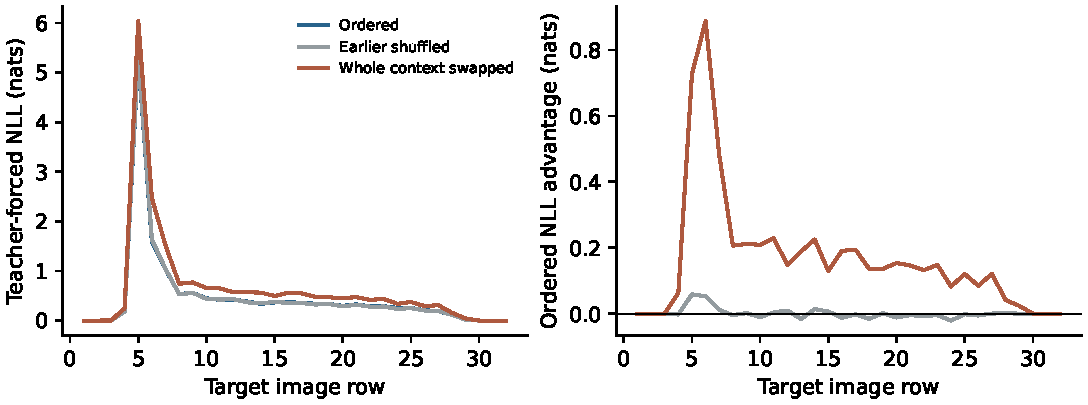
\includegraphics[width=\textwidth]{figures/Figure_S1_context_attribution.pdf}
\caption{\textbf{Exploratory row-wise attribution of raster likelihood.}
Left, teacher-forced NLL by target-image row for ordered, earlier-shuffled and
completely deranged conditions on 512 windows. Right, ordered advantage
relative to each control. Earlier target pixels are legitimately observed by
the image density, so low later-row NLL cannot itself establish language
information from the prompt. Curves are descriptive means; whole-image
uncertainty is reported in Supplementary Note 12.}
\label{fig:context-attribution}
\end{figure}

\section*{Supplementary Note 13: matched joint likelihood learning}
The joint experiment (V55) retains the exact V54 network and probability law.
Both arms initialize from its EMA, with new optimizers and EMA copies. The
frozen control trains only the 2,434,592 density parameters. The joint candidate
also trains reader parameters through the exact image likelihood, for
18,711,840 participating parameters. The unused scalar contrastive temperature
is fixed. Runtime size stays 18,711,841 in both. Reader dropout remains disabled
in both arms, independently of gradient flow. The deployed student continues
to receive and generate image tensors, without a vocabulary or external model.

Each arm makes 8,000 updates with eight streams and 16 selected causal
positions per stream, using 25\% supplied-image motor exercises. Training seed
20265510 and dataset seed 20265511 give matched new draws from the same public
corpus. Both final training-generator states match exactly. The frozen reader
is bit-identical to initialization; the joint reader changes. Reader likelihood
gradients are finite and nonzero only in the joint arm. A four-step interrupted
smoke reproduces every model and EMA tensor, plus CPU/CUDA/training RNG states.
Reader gradients cannot pass through answer-supplied motor rows because those
replace the natural state with a zero hidden vector and a fixed observed field.

The density learning rate is $2\times10^{-4}$ in both arms; joint reader rate
is $2\times10^{-5}$. Other optimizer, warmup, cosine, clipping, BF16 and EMA
settings match the earlier density experiment. The control takes
\ControlTime\ s at \ControlMemory\ GiB allocated CUDA memory; the joint arm
takes \JointTime\ s at \JointMemory\ GiB. Both run sequentially on physical
GPU 0. These costs exclude V42/V54 pretraining and data preparation.

Both checkpoints finish before either development result opens. The same
512 NLL windows, 256 generation/motor prefixes and 64 four-step feedback
streams use audit seed 20265420. Joint ordered NLL is \JointNll\ nats per
image versus \ControlNll\ for the matched frozen control. The paired gain is
\JointNllGain\ nat, interval [\JointNllLow, \JointNllHigh]. The joint-minus-control
sample identity gain is 1.172 percentage points, interval [-0.397, 2.893].
All intervals use 2,000 source-record bootstrap draws. Joint earlier-history
advantage is 0.185 nat [0.128, 0.244], versus 0.119 [0.052, 0.186] for the
continued frozen arm. Extra training accounts for part of the likelihood
progress; the matched gain isolates the reader update's additional benefit.

\section*{Supplementary Table 3: matched learning audit}
\begin{center}\begin{tabular}{lrrrr}\toprule
Arm / decoding & Identity (\%) & Exact image (\%) & Pixel F1 & Isolated ink \\
\midrule
Frozen / ordered & 2.344 & 1.953 & 0.3643 & 0.0070 \\
Frozen / shuffled & 2.344 & 1.953 & 0.3638 & 0.0071 \\
Frozen / greedy & 6.641 & 6.641 & 0.2296 & 0.0028 \\
Joint / ordered & 3.516 & 3.516 & 0.3620 & 0.0074 \\
Joint / shuffled & 3.125 & 3.125 & 0.3625 & 0.0065 \\
Joint / greedy & 7.422 & 7.422 & 0.2230 & 0.0024 \\
\bottomrule\end{tabular}\end{center}
Both arms use 256 paired prefixes and the same post-generation evaluator bank. No sampled output is selected or replaced.


Both arms preserve exact greedy copying on 256/256 targets. Stochastic-copy
F1 is 0.99993 frozen and 0.99994 joint; exact-image match is 96.875\% and
97.266\%, respectively. Joint four-step feedback identity is 3.125\% ordered
and 1.563\% shuffled; control values are 2.344\% and 2.734\%. The joint arm
passes six of eight unchanged gates, failing sampled quality and the ordered
generation advantage. The control passes five, additionally failing feedback.
The matched decision remains \texttt{\JointDecision}. Neither the primary
development reuse nor the paired intervals establish independent seed or
sealed-partition generalization.

\begin{figure}[htbp]
\centering
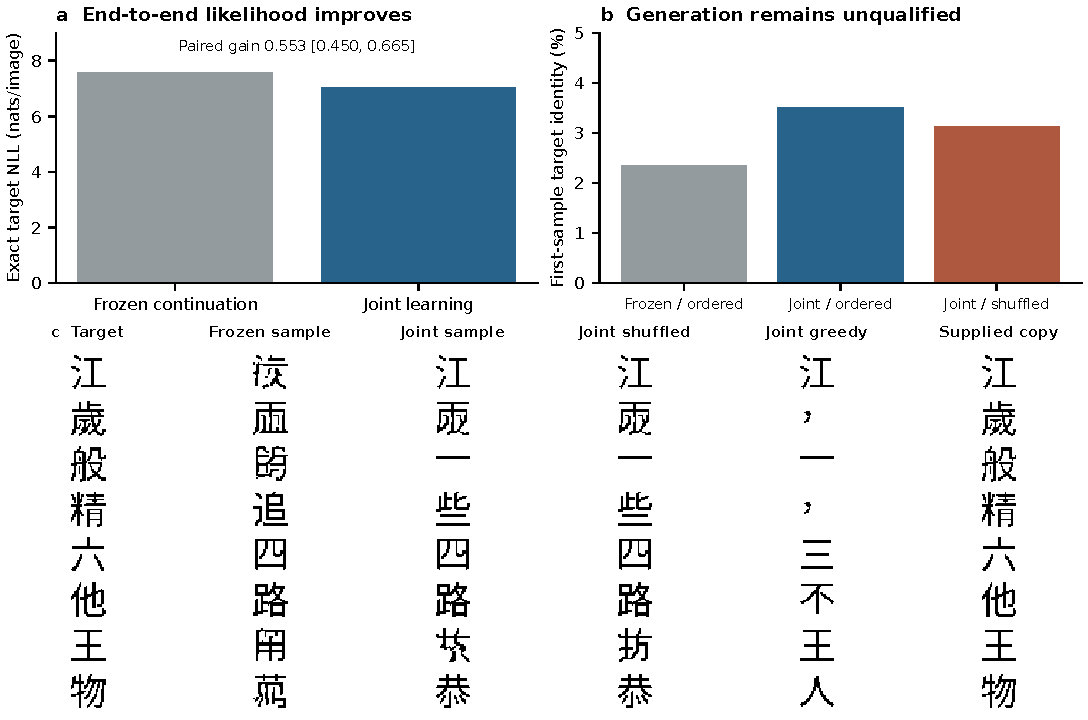
\includegraphics[width=\textwidth]{figures/Figure_S2_joint_learning.pdf}
\caption{\textbf{Matched end-to-end learning of exact raster probability.}
\textbf{a}, Joint reader--density training improves target NLL over the matched
frozen-reader continuation; annotation gives the paired source-record interval.
\textbf{b}, First-sample identity on 256 prefixes remains low under ordered
and earlier-shuffled conditions. \textbf{c}, First eight fixed audit rows:
target, frozen sample, joint sample, joint shuffled sample, joint greedy output
and answer-supplied copying. All outputs are raw model rasters, without
selection, bank replacement or OCR repair. The image panels expose errors that
the likelihood improvement alone cannot resolve.}
\label{fig:joint-learning}
\end{figure}

\section*{Supplementary Note 14: form validity after joint learning}
A post-result diagnostic compares saved images with the same 9,932 distinct
canonical rasters used for evaluation. Exact membership asks whether an output
is a known form; exact target match asks whether it equals the observed next
image. Neither uses nearest-neighbour replacement. The bank is confined to
evaluation and never enters decoding. These descriptive measurements reuse
development outputs and do not change any original decision.

Among 256 first samples, exact known-form membership rises from 9.375\% in
V54 to 33.594\% in the continued frozen arm and 43.750\% in the joint arm.
The paired joint-minus-frozen gain is 10.156 percentage points, with 95\%
source-record interval [4.219, 16.240]. Exact observed-target matches are
0.781, 1.953 and 3.516\%, respectively. In four-step feedback, joint form
membership is 46.875\% versus 38.672\% frozen; the paired gain is 8.203 points
[1.230, 14.683]. The first-sample joint greedy output has 98.438\% membership
but only 7.422\% exact target match and 34 distinct forms, compared with 78
distinct stochastic outputs. Form coherence and linguistic choice remain
separate requirements (Fig.~\ref{fig:form-validity}).

\begin{figure}[htbp]
\centering
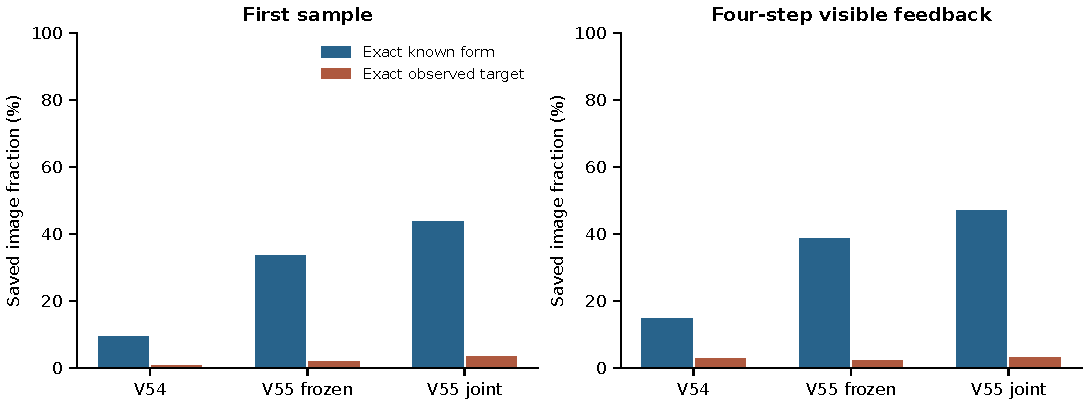
\includegraphics[width=\textwidth]{figures/Figure_S3_form_validity.pdf}
\caption{\textbf{Exact canonical form does not imply correct continuation.}
Saved first samples and four-step feedback images are compared with a fixed
canonical raster bank. Blue bars require exact pixel equality with any known
form; brown bars require equality with the observed future image. All three
checkpoints use the same bank. The paired uncertainty is stated in Note 14;
the bars are descriptive fractions, not independent replications.}
\label{fig:form-validity}
\end{figure}

\section*{Supplementary Note 15: raw-pixel beam decoding}
The V56 decoder changes search alone. V55 joint weights and the complete
binary-image law remain fixed. A beam of eight prefixes expands the next
binary pixel to ink or background, adds its exact conditional log probability
and retains the eight best scores. The row model observes preceding rows;
the masked within-row head observes preceding pixels. Parent gathering keeps
row history and row conditions aligned. Stable ties prefer ink and then the
earlier parent. Width one reproduces the original greedy rule. No persistent
glyph inventory, target identity, image replacement, rejection filter or
external model enters the decoder. Beam eight is approximate mode search,
not exact global maximization over all $2^{1024}$ images.

A two-image numerical preflight found that the original high matmul precision
gave incremental/parallel score differences above the frozen $10^{-3}$-nat
tolerance. An amendment recorded before production sets both beam and greedy
controls to highest FP32 matmul precision. It changes no weights, windows,
beam width, tolerance or quality gate. Production maximum score discrepancy
is $2.10\times10^{-5}$ nat and the width-one equality check passes.

The fixed audit uses 2,048 development windows, seed 20265620, 64 visible cells
and eight future targets. Exact next-image matches are 238/2,048 for ordered
beam, 202/2,048 for earlier-shuffled beam and 169/2,048 for ordered greedy:
\BeamAccuracy, \BeamShuffled\ and \GreedyAccuracy\%, respectively. Shuffling
preserves the final four visible cells. The paired beam-minus-greedy gain is
\BeamGain\ points [\BeamGainLow, \BeamGainHigh]; ordered-minus-shuffled is
\BeamHistoryGain\ points [\BeamHistoryLow, \BeamHistoryHigh]. Intervals use
2,000 source-record bootstrap draws, seed 20265719, with 188 source records.
All ordered and shuffled beam outputs exactly match a known canonical form.
The post-generation bank has 9,934 distinct rasters and covers every target;
it is descriptive, not the search space. Beam emits 127 distinct first forms,
versus 116 greedy. Its mean self NLL is 3.108 versus 3.508 nats/image; this
scores the selected output, not the true target, and is not a training gain.

Visible feedback uses the first 128 prefixes for eight steps. Exact observed
image matches are 68/1,024 ordered beam, 51/1,024 shuffled beam and 50/1,024
greedy. The beam-minus-greedy difference is 1.758 points [0, 3.770], with 89
source records. Adjacent image repetition is 228/896 transitions
(\BeamRepeat\%) for beam, versus one transition (\TargetRepeat\%) in the
observed streams. Shuffled beam repeats 32.366\% and greedy 17.746\%.
Mean distinct images per eight-step stream are 4.711 beam and 7.789 observed.
Thus search improves immediate conditional choice while longer output remains
repetitive (Fig.~\ref{fig:pixel-beam}). Five of six gates pass; feedback
repetition fails and the decision is \texttt{\BeamDecision}.

All 256 supplied motor images still copy exactly. The audit takes
\BeamSeconds\ s with \BeamMemory\ GiB peak allocated CUDA memory on GPU 0,
excluding previous training and data preparation. No new training or sealed
evaluation is performed. This bounded search result does not establish
question answering, instruction following, historical-script generation or
capability-matched efficiency against a text language model.

\begin{figure}[htbp]
\centering
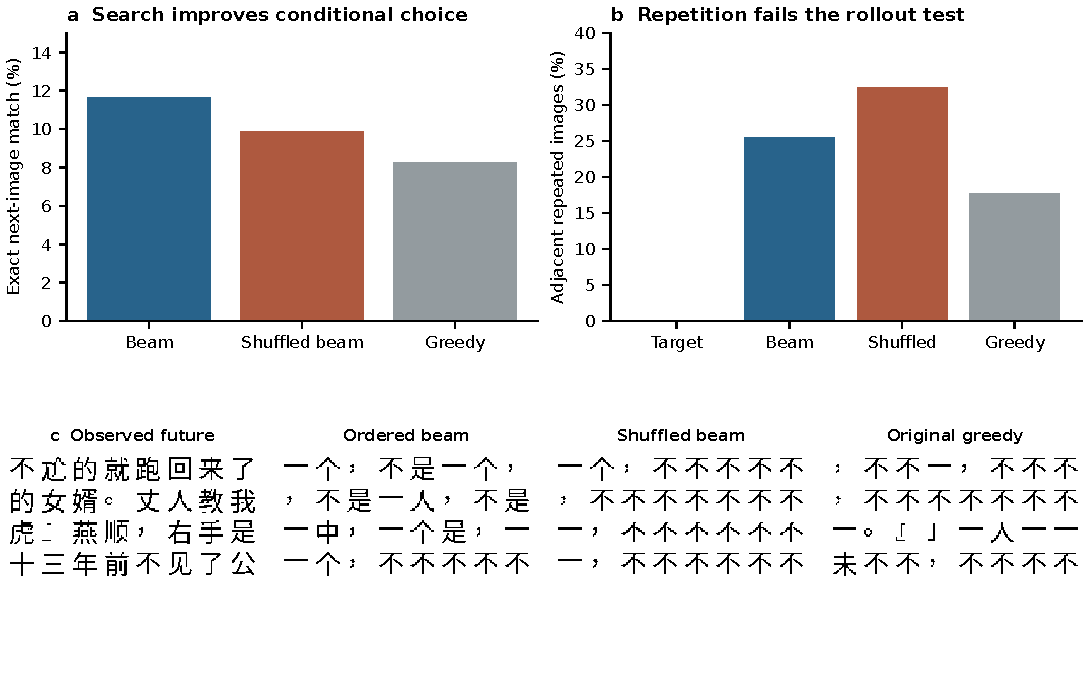
\includegraphics[width=\textwidth]{figures/Figure_S4_pixel_beam.pdf}
\caption{\textbf{Pixel search improves next-image choice but fails rollout.}
\textbf{a}, Exact target-image matches on 2,048 fixed prefixes, with unchanged
weights across ordered beam, earlier-shuffled beam and greedy controls.
\textbf{b}, Adjacent raster repetition over eight-step feedback, compared
with observed future streams. \textbf{c}, First four fixed audit streams:
observed future and raw generated images. No examples are selected or repaired.
Paired intervals are reported in Note 15; the feedback failure remains the
decoder's qualification decision.}
\label{fig:pixel-beam}
\end{figure}

\section*{Supplementary Note 16: grounded image-answer learning}
The V57 model retains the V55 joint reader and exact raster writer, extending
the allowed causal context from 64 to 512 cells. Parameter-free rotary
positions require no weight-shape change; this extension does not itself
establish trained long-context competence. Two $384\times384$ projections
produce source-position attention from the final causal query and observed
prompt states. A linear copy gate and a linear stop head give 295,682 new
parameters, for 19,007,523 runtime parameters. The contrastive temperature
remains unused and fixed. Both reader and density continue learning.

For observed source images $X_i$, attention $a_{ti}$ and copy gate
$\lambda_t$, the continued image distribution is
\begin{equation}
q_t(Y)=\lambda_t\sum_i a_{ti}\mathbf{1}[Y=X_i]
       +(1-\lambda_t)r_t(Y).
\end{equation}
Here $r_t$ is the normalized exact raster density. Duplicate source images
contribute summed mass. Equality uses lossless bit packing of observed binary
pixels; there is no persistent symbolic identity or writing bank. A query
cannot attend to source positions later than itself, including when natural
training sequences are packed together. With stop hazard $s_t$,
$p_t(\mathrm{stop})=s_t$ and
$p_t(Y,\mathrm{continue})=(1-s_t)q_t(Y)$. Training includes the terminal stop
event after a reference answer. Reference length determines supervision masks,
not a deployed input. Runtime receipts retain an inherited Bernoulli-density
description; it describes $r_t$ alone, not the complete mixture/event law.

CMRC 2018 supplies natural questions over Wikipedia paragraphs\cite{cmrc}.
Pinned source revision and original annotation offsets are checked during data
preparation. Whitespace is removed consistently, unsupported font forms are
excluded, full rendered prompts are limited to 480 cells and retained answers
to 16. No answer-centred crop is used. Answers must match the source substring
and not occur verbatim in the question. The result contains 3,211 training
questions over 1,134 paragraphs and 1,321 development questions over 421
paragraphs. Article-title and context-hash overlap are zero across splits.
The data retain CC-BY-SA-4.0 attribution. Canonical rendering and thresholding
match V55. No symbolic label is passed to a student method.

Both arms initialize from the same V55 EMA, train for 4,000 updates with batch
four and use identical data RNGs. Three of four updates draw uniform training
questions with replacement; the fourth retains 16 causal positions per natural
stream, including 25\% supplied-image motor conditions. Motor conditions use
zero hidden states and exact observed fields, bypass copying and omit the stop
loss. The no-copy arm fixes $\lambda=0$; its source-attention heads are frozen.
The first retained answer supervises event likelihood, while evaluation accepts
every retained reference. Loss is mean exact event NLL over valid image and
stop events, without the earlier image-only $1/1024$ rescaling.

AdamW rates are $3\times10^{-5}$ for the reader, $10^{-4}$ for the density and
$3\times10^{-4}$ for new heads; betas are (0.9,0.95), weight decay 0.01,
warmup 200 updates, cosine decay to 10\%, norm clip one and EMA 0.999. BF16
training uses deterministic CUDA algorithms, math SDPA and fixed cuBLAS
workspace configuration; reader dropout stays disabled. A four-update smoke
matches interrupted two-plus-two training exactly for all model/EMA tensors
and data, training, CPU and CUDA RNG states. A masked-copy backward regression
test covers matches occurring only at forbidden future positions. Copy and
no-copy training take \QaSeconds\ and \QaControlSeconds\ s, with
\QaMemory\ and \QaControlMemory\ GiB peak allocated CUDA memory on GPU 0.
These costs exclude previous foundation training and preparation.

Both final EMA checkpoints complete before development opens. Primary IDs are
256 samples without replacement from sorted development records, seed
20265720. The decoder stops at hazard $\geq0.5$; otherwise it selects the copy
component at gate $\geq0.5$, sums attention over equal observed rasters and
emits the largest-mass image. The free component uses pixel beam eight. This
is hierarchical greedy decoding, not global mixture-mode search. The 17-cell
safety cap is recorded separately from stopping. No answer location, reference
length or candidate answer list is available at inference.

Exact answer match requires every output image, its order and learned stop to
match a retained reference. Raster F1 measures multiset overlap of exact
rasters, maximizing over references. It can credit reordered images and is
not the official word-segmented CMRC metric. Primary copy exact match is
10/256 (\QaExact\%), versus 1/256 with question pixels blanked and 0/256 no-copy. Copy F1 is
\QaFone\%, versus \QaBlankFone\% and \QaControlFone\%. Its paired gain over
blanking is \QaQuestionGain\ points [\QaQuestionLow, \QaQuestionHigh]; over
no-copy it is 9.136 [5.879, 12.483]. Intervals use 2,000 source-article draws,
seed 20265819, retaining related questions together (198 primary articles).
The blanking intervention removes question ink while retaining passage and
framing; it is not an in-distribution alternative natural question.

All 393 shared-paragraph/disjoint-answer question pairs are also tested.
Only one has both answers exactly correct (\QaPairExact\%). Mean primary
answer length is 10.457 cells, and 58/256 cases reach the safety cap.
Every primary copy-arm image uses copying, with no free-branch emission.
Teacher-forced mean event NLL across all 1,321 development questions is
1.329 copy versus 12.025 no-copy; mean sequence NLL is 8.377 versus 91.477.
All 256 V55 supplied motor images remain exact. The full audit takes
1,117.1 s and peaks at 0.140 GiB allocated CUDA memory, including the slower
2,106-image free-writing control. Four of seven gates pass: boundary, clean
split/resources, motor and question-dependent F1. Exact answers, absolute F1
and paired-question correctness fail. The decision is \texttt{\QaDecision}.

A post-result, zero-model-call diagnostic on the saved primary outputs finds
43/256 correct first images. Only 10/43 of those become exact complete answers;
14/256 outputs contain a complete reference prefix followed by unwanted
additional images. Mean aligned correct prefix length is 0.750 cells; adjacent
repetition is 2.230\%. These descriptive observations do not alter the locked
decision. They motivate testing answer-level structure alongside better
evidence selection. All results remain limited to canonical, answerable,
short-paragraph reading; independent seed replication, raw page segmentation,
historical writing and general language generation are unestablished.

\section*{Supplementary Note 17: complete observed image blocks}
V58 continues the completed V57 copy EMA with a normalized distribution over
all contiguous observed prompt blocks $X_{i:j}$, where $1\leq j-i+1\leq16$.
For causal states $h_i$ and final prompt state $h_L$, define
\[
 s_{ij}=\frac{(W^s_qh_L)^\top W^s_kh_i+
                   (W^e_qh_L)^\top W^e_kh_j}{\sqrt{384}}+b_{j-i+1},
 \qquad \pi_{ij}=\frac{e^{s_{ij}}}{\sum_{uv}e^{s_{uv}}}.
\]
The answer-image law is
\[
 p(Y\mid X)=\sum_{ij:\,X_{i:j}=Y}\pi_{ij}.
\]
Equality is lossless raster equality, computed from binary pixels; indices
address only the current prompt. There is no persistent glyph inventory.
Training minimizes exact negative log block mass, divided by reference cell
count plus one boundary event across the batch. Annotated source offsets do
not enter the loss. Mode decoding sums mass over equal sequences and chooses
the most probable sequence, with first-source tie breaking. No reference
length, answer list, OCR or output repair enters generation. The predicted
end boundary terminates a nonempty block; the 16-cell support is fixed before
training. The retained copy/free/stop continuation path remains separate.

Four new 384-by-384 projections and sixteen length biases bring the runtime
to 19,597,363 parameters. Projection pairs initialize from V57 copy attention;
the matched glyph control constructs and freezes the same new heads. Both
start from identical V57 copy EMA weights and make 4,000 updates, batch four,
using the previous three-to-one QA/natural-motor schedule, optimizer rates
and deterministic settings. Seeds are 20265810 (training) and 20265811 (data).
A four-update uninterrupted versus two-plus-two resumed GPU run matches all
model/EMA tensors and data, training, CPU and CUDA RNG states exactly.
Block training takes 210.995 s, 0.967 GiB peak allocated memory; the glyph
control takes 302.237 s, 1.056 GiB. Earlier foundation costs are excluded.

Both final checkpoints precede development inspection. Primary IDs are the
same 256 as V57, explicitly reused development, not a sealed final test.
Exact answers are 25/256 (9.766\%) block, 3 blank-question and 21 matched glyph control.
F1 is 27.033\%, 9.169\% and 22.140\%. Article-grouped bootstrap uses 2,000
draws, seed 20265919. Block-minus-control F1 is 4.893 points [0.469, 9.047];
exact match is 1.563 [-1.509, 4.652]. Normal-minus-blank F1 is 17.864
[13.438, 22.289]. Only 4/393 pairs have both answers correct; the paired gate
fails and the registered decision remains \texttt{reject\_reading\_model}.
All 256 supplied motor images remain exact. Mean conditional block sequence
NLL is 6.505, versus 9.552 for glyph-event sequence likelihood; these laws have
different supports and must not be treated as interchangeable language
perplexities. The audit takes 98.951 s at 0.142 GiB allocated memory.
The 78,772,107-byte inference-only export reproduces native prompt-PNG
answers and events exactly. Raw first audit failures appear in Figure 5.

\section*{Supplementary Note 18: frozen visual foundation probe}
V59 pins MIXAR-477M stage-2 revision
\texttt{c5d5bcfbad2f290296fd83810558f396c6a6333a}, reusing its shared
Apache-2.0 checkpoint. Author-reported multilingual pretraining and its
four-H200 compute are external work, not part of single-4090 training here.
Both it and the frozen V58 reader consume identical Noto CJK 26-pixel glyphs
inside binary 32-pixel cells. This differs from MIXAR's native rendering.
An odd-length prompt gets a blank final cell for two-cell pairing; readout
candidates exclude that extra cell. Both encoders supply states after each
complete pair, repeated over its two source cells.

A fixed CPU-QR semi-orthogonal projection maps MIXAR's 896 states to 384
coordinates, seed 20265900; student states already have width 384. Both append
128 projected normalized-DCT coordinates, seed 20265901, plus two within-pair
phase channels. Semantic and fine-image parts are separately RMS-normalized.
The 514-dimensional features are quantized to FP16 for caching and readout.
All train, development and blank-question features are prepared without
reading answer annotations. Recomputed quantized features agree exactly.

Each fresh head has four 514-to-384 projections and sixteen biases, totaling
789,520 learned parameters. Both train 4,000 updates, batch eight, with seeds
20265910/20265911, AdamW rate $3\times10^{-4}$, betas (0.9,0.95), decay 0.05,
norm clip one, warmup 200, cosine to 10\%, and EMA 0.999. Frozen encoders and
native free writers are unchanged. An interrupted/resumed GPU preflight
matches weights, EMA and RNG states exactly. Features take 184.781 s and
1.906 GiB; student and MIXAR readouts take 106.593 and 109.257 s, each at
0.170 GiB. These resource numbers exclude external pretraining.

Both completed heads precede inspection of the same reused 256 development
IDs and 393 pairs. Student exact/F1 scores are 9.375/25.340\%; MIXAR scores
2.344/11.588\%. MIXAR-minus-student F1 is $-13.752$ points
[$-18.247$,$-9.094$], using 2,000 article draws, seed 20266019.
Normal-minus-blank F1 is 2.246 [0.415,4.378] for MIXAR, versus 18.343
[13.949,22.519] for the student. Both questions are exact in zero versus
twelve pairs. Three of seven gates pass; the frozen-foundation probe fails.
The 117.085-s, 0.094-GiB audit uses cached readouts and excludes online encoder
inference. Figure S5 reports all four conditions. Capacity, pretraining,
prior task training and rendering differ; this is a scoped foundation probe,
not a general ranking of encoders or native-font MIXAR competence.

\plate{Figure_S5_frozen_foundations}{\textbf{Frozen pretrained features do not
improve this reading interface.} Identical learned block heads consume frozen
student or MIXAR features, with normal and blank-question prompts. All scores
use the fixed 256 questions. External pretraining and rendering shift prevent
a causal attribution to capacity or pretraining alone.}{fig:frozen-foundations}

\section*{Supplementary Note 19: question-first causal reading}
V60 tests whether passage states should be conditioned on the question before
evidence selection. The context-first host layout places passage $X$ before
question $Q$; the intervention reverses these two blocks, yielding causal
passage states $h_i=f(Q,X_{\leq i})$. Framing and total visible length are
unchanged. Both models start from identical V58 block EMA weights and retain
the 19,597,363-parameter architecture, block law, image-only supervision,
mode decoder and continuation writer. All visible prompt positions remain
candidates. There is no answer offset or answer-aware cropping.

Each arm makes 4,000 updates with the same V58 batch-four schedule, optimizer
rates, warmup, cosine, clipping, EMA and deterministic BF16/math-SDPA regime.
Training/data seeds are 20266010/20266011. The new prompt-order helper is
tested for exact preservation of source characters and correct blanking
positions. An uninterrupted versus two-plus-two resumed GPU preflight
matches all model/EMA tensors and RNG states exactly. Both production arms
finish before their development scores open. Context-first and question-first
training take 214.699 and 225.207 s, each at 0.966 GiB peak allocated CUDA
memory. Cost remains incremental to the same previously trained foundation.

The same 256 primary IDs and 393 paragraph pairs are explicitly reused.
Question pixels are blanked at each arm's actual question positions, retaining
the paragraph, length and framing. Exact answers are 27 context-first and
21 question-first, versus three and two for the corresponding blank controls.
F1 is 26.908\% and 23.765\%, versus 7.572\% and 9.098\% blanked. With 2,000
article-grouped bootstrap draws, seed 20266119, question-first minus
context-first F1 is $-3.143$ points [$-6.544$,0.446]; exact match is
$-2.344$ [$-5.490$,0.810]. Neither difference resolves zero. The question-first
normal-minus-blank F1 gain is 14.667 [10.873,18.809]. Both answers are exact in
5/393 question-first pairs, versus 16/393 context-first pairs.

All 256 supplied motor images remain exact for both arms. The complete audit
takes 192.723 s at 0.184 GiB allocated CUDA memory. Four of eight registered
gates pass: boundary, clean split/resources, question-dependent F1 and motor.
The gain, absolute accuracy, absolute F1 and paired-question gates fail, so
the decision is \texttt{reject\_question\_first\_intervention}. This is one
matched training seed and a task-trained, context-first foundation; neither a
universal ordering result nor a final generalization test is established.

\plate{Figure_S6_question_first}{\textbf{Changing input order is insufficient.}
Matched models receive the same source writing with the question before or
after the passage. Question blanking uses each layout's actual positions.
The question-first F1 difference is unresolved and its registered reading
criteria fail.}{fig:question-first}

\section*{Supplementary Note 20: full native pixel-language adaptation}
The complete released MIXAR-477M\cite{mixar} image-language model is adapted
using the pinned release identified by its full revision, weight SHA-256 and
architecture-code hashes in the accompanying evidence. This is
supervised adaptation of external pretraining, not local foundation training
from scratch. All 477,145,984 contextual and image-output parameters train.
The source data are the same 3,211 training and 1,321 development questions
used for the preceding reading experiments, with no article or context-hash
overlap. Development is explicitly reused. Complete prompts contain at most
480 cells and first-reference training answers at most 16 cells.

Noto CJK glyphs at 26 pixels occupy 32-pixel binary cells, a rendering shift
from the author's native bundled-font interface. Odd prompt/answer lengths
receive one blank cell for alignment to 32-by-64 native blocks. Two all-white
blocks follow each target answer. Native input uses white $+1$ and ink $-1$;
the target Bernoulli probability describes white pixels. Spatial prompt bounds
are known, but strings, codepoint IDs and source-answer offsets never enter
the actor. The causal answer-only objective is
\begin{equation}
\mathcal L=-\frac{1}{|A|P}\sum_{t\in A}\sum_{i=1}^{P}
\left[y_{ti}\log\sigma(a_{t-1,i})+(1-y_{ti})\log(1-\sigma(a_{t-1,i}))\right],
\end{equation}
where $P=2048$, $A$ contains answer and termination blocks, and state $t-1$
depends only on preceding physical images. Prompt labels contribute no loss.

The registered run uses 1,000 updates, microbatch one accumulated eight times,
uniform replacement sampling, AdamW $2\times10^{-5}$, betas $(0.9,0.95)$,
weight decay 0.01, warmup 50, cosine decay to 10\%, norm clip one and EMA
0.99. Seeds are 20266110 for training and 20266111 for data. FP32 weights,
optimizer and EMA coexist with BF16 forward/backward, deterministic algorithms,
math attention and nonreentrant activation checkpointing. The final EMA is
used without development checkpoint selection. A real four-update interrupted
preflight reproduces model, EMA, optimizer and all RNG states exactly, with
finite gradients throughout. Altering future answer pixels changes earlier
logits by exactly zero in the recorded causality check.

Training through the final update takes 1,501.138 s, with 9.912 GiB peak
allocated memory; loading takes 2.525 s. Cache preparation, final serialization
and external pretraining are separate. All work uses physical GPU 0. Greedy
decoding thresholds each white logit at zero, feeds back the generated image
and stops at the first exactly white block, otherwise capping at ten new
blocks. Only terminal blocks and entirely blank trailing cells are removed.
No malformed image is repaired or snapped to a character.

The locked audit compares adapted and released-base actors with normal and
blank-question inputs on the same 256 primary IDs, and tests all 393
shared-paragraph question pairs for the adapted actor. All 1,321 development
examples contribute likelihood. Pixel NLL decreases from 0.684156 to
0.154814 nats, yet exact answers are zero and exact-raster multiset F1 is
0.149\%. Foreground F1 is 12.264\%, compared with 8.473\% blanked and zero
for the released base under this shifted interface. Article-grouped bootstrap
with 2,000 draws, seed 20266219, gives the adapted-minus-blank foreground
difference as 3.791 points [2.521,5.056]. The exact-raster F1 difference is
0.149 [0,0.372], unresolved. Both-correct pair accuracy is 0/393.

No primary output is empty or capped for the adapted actor; the released base
returns an empty answer on every normal primary prompt. The adapted mean
length is 3.047 cells. Five of ten gates pass: image-only runtime, clean
split/finite resources, full backward/resume/causality, independent replay,
and capped-output rate. Exact answers, raster F1, adaptation gain,
question-dependent raster F1 and paired correctness fail. Audit time is
145.690 s excluding loading, at 1.832 GiB allocated memory. The registered
decision is \texttt{reject\_native\_free\_reading}.

A learned-weight deployment bundle includes configuration and local custom
architecture code. A fresh offline process with empty model and code caches
reproduces actual answer tensors, PNG bytes and stopping events. It loads no
original release weights and calls no external model, tokenizer or OCR.
Exact replay is an implementation result, separate from language quality.

An auxiliary transcription plan was registered before development outputs
were inspected. CPU Tesseract 5.3.4 receives anonymous answer-only images,
enlarged fourfold with a white margin, without questions, references or model
names. It recognizes only 40/256 retained reference images exactly, a 15.625\%
calibration rate. No generated answer is transcribed exactly, but the poor
reference calibration precludes treating this as a reliable semantic score.
The primary raw-image failure and strict gates remain unchanged. One seed,
the shifted font interface, limited training data and absent general-language
evaluation constrain the interpretation.

\section*{Supplementary Note 21: conditional whole-image density}
The matched experiment tests a latent expert shared across a complete native
image block. Let $h_t$ be the visual transformer's causal state after the
visible prefix and let $y\in\{0,1\}^{2048}$ denote the next $32\times64$
bitmap, with one denoting white in this native interface. The normalized law is
\begin{equation}
 p_\theta(y\mid h_t)=\sum_{k=1}^{K}\pi_{\theta k}(h_t)
 \prod_{i=1}^{2048}q_{\theta ki}(h_t)^{y_i}
 [1-q_{\theta ki}(h_t)]^{1-y_i},
 \qquad q_{\theta ki}=\sigma(a_{\theta ki}),
\end{equation}
where the gate is a softmax. Each expert is a neural function of the current
visual state, without a fixed character identity or stored target bitmap.
Marginalizing the expert retains a proper probability law. For distinct
pixels, conditional covariance is
\begin{equation}
 \operatorname{Cov}(Y_i,Y_j\mid h_t)
 =\sum_k\pi_k q_{ki}q_{kj}
 -\Bigl(\sum_k\pi_k q_{ki}\Bigr)\Bigl(\sum_k\pi_k q_{kj}\Bigr).
\end{equation}
It can be nonzero even though pixels are independent within one expert.
This elementary property permits coherent alternatives; it does not prove
that training discovers valid writing or useful answers.

The objective is exact negative log joint likelihood, computed with
\texttt{logsumexp}, divided by 2,048 physical pixels. It averages only
answer and two blank termination blocks within each example, then averages
over accumulated examples. Teacher forcing uses the same one-block causal
shift as Note 20. Prompt pixels enter the context without a prompt loss.
There is no transcript, answer-span offset or Unicode target inside the actor.

The single-head control has 477,145,984 parameters; eight experts have
489,998,208. Both initialize from the same externally pretrained MIXAR
revision and use the unchanged Noto-26 cell interface, 3,211 training
questions and 1,321 article-disjoint development questions. The eight-head
projection repeats the released head with zero-mean perturbations of scale
0.01, seed 20266210, and a zero-initialized gate. Every backbone and head
parameter receives gradients. The comparison matches examples, optimization
and update budget, rather than parameter count or output computation.

Each arm uses 1,000 updates, microbatch one, accumulation eight, AdamW at
$2\times10^{-5}$ with betas $(0.9,0.95)$, decay 0.01, 50-update warmup,
cosine decay to 10\%, norm clip one and EMA 0.99. Weights, optimizer and EMA
are FP32; forward/backward use BF16 with deterministic algorithms, eager/math
attention and nonreentrant activation checkpointing. Training and data seeds
are 20266220 and 20266221. Complete sampled-example orders must match exactly.
Only the final EMA is audited. Both arms run sequentially on physical GPU 0,
under a 20 GiB allocated-memory and four-hour ceiling per phase.

Generation thresholds each expert into one complete candidate bitmap, scores
all candidates under the full mixture and emits the highest-scoring candidate.
Searching component modes is approximate MAP; it is not a guarantee of the
global mixture mode. Actual emitted pixels become subsequent context. The
first exactly white native block ends generation, otherwise ten blocks cap
the continuation. Only the detected terminal block and wholly blank trailing
cells are removed. Malformed nonblank strokes are preserved. The deployed
bundle has no tokenizer, OCR, glyph inventory or external language-model call.

The primary audit retains the fixed 256 questions, blank-question controls,
all 393 shared-paragraph pairs and all-development likelihood. Paired
intervals resample articles 2,000 times, seed 20266229. An intervention pass
requires positive lower intervals for both K8-minus-K1 strict-raster F1 and
K8 normal-minus-blank F1, fewer than 20\% capped outputs and all implementation
checks. Each arm's separate bounded reading gate requires at least 10\%
exact answers, 25\% raster F1, 2\% both-correct pairs, a positive question
effect, fewer than 20\% caps and implementation checks. Expert-use counts
and gate entropy are descriptive; they cannot select a new checkpoint or
change these gates. Reused development, one seed, the shifted font interface
and external pretraining limit the conclusions.

Both arms complete their registered budget and all replay checks. K=1 takes
1,887.5 s at 9.904 GiB peak allocated memory; K=8 takes 1,972.8 s at 10.174 GiB.
Their complete training-example orders match exactly. The locked audit takes
527.4 s excluding model loading, at 1.904 GiB allocated memory. Four-update
uninterrupted versus two-plus-resumed-two preflights match model, EMA,
optimizer and every RNG state exactly for each arm. Future-pixel changes
have zero effect on earlier predictions. Strict-FP32 cache errors remain
below $2.1\times10^{-5}$; larger TF32 discrepancies are retained separately
rather than hidden by changing the production recipe.

All-development NLL is 0.1542 for K=1 and 0.1248 for K=8. Primary strict-raster
F1 is 0.234\% versus 0.815\%, a 0.580-point gain [0.089, 1.094]. Foreground
F1 is 12.205\% versus 15.827\%, a 3.623-point gain [1.815, 5.554]. Both
arms have zero exact primary answers and zero both-correct pairs. K=8's
normal-minus-blank raster difference is 0.295 points [$-0.006$, 0.623]; its
foreground difference is $-0.044$ points [$-0.629$, 0.509]. Neither resolves
question dependence. Seven of eight intervention gates pass; both arms pass
six of ten bounded reading gates. The registered decision is
\texttt{reject\_density\_intervention}; neither arm qualifies as free reading.

K=8 selects experts 0, 1, 2, 4 and 7 on respectively 223, 4, 106, 605 and 3
primary generation steps, including termination. Mean gate entropy is 1.812
nats, compared with $\log 8=2.079$ for a uniform gate. The primary outputs all
terminate before the cap, while one blank-question output reaches the cap.
These descriptive observations do not identify semantic expert roles or
justify selecting different parameters. The result supports improved bitmap
fit at this budget, while the required question-dependent language remains
unestablished.

\subsection*{Auxiliary reader and post-hoc transcript sensitivity}
A separately preregistered, answer-only Qwen3-VL 8B reader transcribes
122/128 training-reference images exactly (95.313\%), returns every one of
16 blank and 16 random-ink controls empty, and produces valid JSON throughout
calibration. The fixed instruction and anonymous images disclose neither
questions nor reference answers to the reader. Three responses among 1,015
unique actor images are invalid, including two that reach the registered
256-output-token limit. The original diagnostic therefore reports
\texttt{invalid\_actor\_transcription}; it has no complete fixed-case score.

An explicitly post-hoc sensitivity analysis reuses the first responses
without retry, repair or new model calls. It retains all 256 cases in each
condition and assigns each invalid bounded score possible range $[0,1]$.
The resulting full-case means are below; ranges are identification intervals,
not confidence intervals. Exact text means normalized transcript agreement
with any retained reference. Character score is one minus normalized edit
error, clipped to $[0,1]$.
\begin{center}\small
\begin{tabular}{lrrr}\toprule
Condition & Valid / unknown & Exact text (\%) & Character score (\%)\\\midrule
K=1 & 254 / 2 & 0.781--1.563 & 1.388--2.169\\
K=1, blank Q & 255 / 1 & 0.000--0.391 & 0.186--0.577\\
K=8 & 256 / 0 & 0.000 & 2.806\\
K=8, blank Q & 256 / 0 & 0.000 & 2.945\\
\bottomrule\end{tabular}
\end{center}

K=8's normal-minus-blank character difference is $-0.139$ percentage points,
with article-bootstrap sensitivity envelope [$-0.962$, 0.638]. The envelope
uses 2,000 article resamples, seed 20266379, taking the lower endpoint's
2.5th percentile and upper endpoint's 97.5th percentile. It covers the
unknown-score assignments within this resampling scheme, not systematic
reader errors, training-seed variation or reused-development selection.
It establishes no new model qualification and changes neither failed decision.
The external reader makes 1,172 calls over 1,092.1 s of owned runtime including
cleanup; maximum resident GPU memory sampled after requests is 7,278 MiB.
These costs are separate from actor inference and training. The evaluator
server and runner exit, its port closes and GPU 0 memory is released.

\section*{Reproduction}
From the repository root, use the following entry points. All use only GPU 0.
\begin{quote}\small\ttfamily
CUDA\_VISIBLE\_DEVICES=0 PYTHONPATH=. python\\
scripts/train\_causal\_visual\_block\_diffusion\_v53.py --device cuda:0
\end{quote}
\begin{quote}\small\ttfamily
CUDA\_VISIBLE\_DEVICES=0 PYTHONPATH=. python\\
scripts/eval\_causal\_visual\_block\_diffusion\_v53.py --device cuda:0
\end{quote}
Completed output directories are protected against accidental replacement.
For the exact density, with the same GPU selection, use
\begin{quote}\small\ttfamily
scripts/train\_exact\_raster\_density\_v54.py\\
scripts/eval\_exact\_raster\_density\_v54.py
\end{quote}
Independent image inference and export use
\begin{quote}\small\ttfamily
scripts/infer\_exact\_raster\_density\_v54.py.
\end{quote}
For the matched continuation, run the following with \texttt{--arm frozen}
and then \texttt{--arm joint}, completing both before the evaluator:
\begin{quote}\small\ttfamily
scripts/train\_joint\_exact\_raster\_v55.py\\
scripts/eval\_joint\_exact\_raster\_v55.py
\end{quote}
The independent runtime uses
\texttt{scripts/infer\_joint\_exact\_raster\_v55.py}.
The form diagnostic and locked pixel decoder audit use
\begin{quote}\small\ttfamily
scripts/diagnose\_raster\_form\_validity.py\\
scripts/eval\_raster\_beam\_v56.py.
\end{quote}
Independent pixel-beam inference uses
\texttt{scripts/infer\_raster\_beam.py}.
For grounded visual reading, complete both training arms before auditing:
\begin{quote}\small\ttfamily
scripts/train\_visual\_copy\_language\_v57.py --arm copy\\
scripts/train\_visual\_copy\_language\_v57.py --arm no\_copy\\
scripts/eval\_visual\_copy\_language\_v57.py.
\end{quote}
Native answers and self-contained export use
\begin{quote}\small\ttfamily
scripts/infer\_visual\_copy\_language.py.
\end{quote}
For complete image blocks, train both arms before the audit:
\begin{quote}\small\ttfamily
scripts/train\_visual\_answer\_blocks\_v58.py\\
scripts/eval\_visual\_answer\_blocks\_v58.py.
\end{quote}
Native inference uses
\begin{quote}\small\ttfamily
scripts/infer\_visual\_answer\_blocks.py.
\end{quote}
Frozen-feature preparation, matched readout training and audit use the
\texttt{cache\_frozen\_visual\_features\_v59},
\texttt{train\_frozen\_visual\_readout\_v59} and
\texttt{eval\_frozen\_visual\_readout\_v59} scripts.
The matched input-order experiment runs both orders before auditing:
\begin{quote}\small\ttfamily
scripts/train\_question\_first\_reading\_v60.py\\
--order context\\
--order question\\
scripts/eval\_question\_first\_reading\_v60.py.
\end{quote}
Native pixel preparation, full adaptation and locked audit use the existing
Python 3.12 MIXAR runtime, with \texttt{CUDA\_VISIBLE\_DEVICES=0}:
\begin{quote}\small\ttfamily
scripts/prepare\_native\_pixel\_qa\_v61.py\\
scripts/train\_native\_pixel\_instruction\_v61.py\\
scripts/verify\_native\_pixel\_export\_v61.py\\
scripts/eval\_native\_pixel\_instruction\_v61.py.
\end{quote}
Independent image inference uses
\texttt{scripts/infer\_native\_pixel\_language.py}.
The matched whole-image experiment uses the persistent sequential coordinator
\begin{quote}\small\ttfamily
scripts/run\_correlated\_native\_v62.py.
\end{quote}
It verifies both complete training reports, standalone offline replays and
the locked audit in that order. Independent image inference uses
\texttt{scripts/infer\_correlated\_native\_language.py};
the exported bundle's \texttt{run.py} does not need the repository or the
original foundation checkpoint. The optional, separately calibrated vision
diagnostic is \texttt{scripts/audit\_correlated\_native\_transcripts\_v62.py}.
That reader stays outside the actor and changes no primary gate.
\begin{thebibliography}{14}
\interlinepenalty=10000
\bibitem{pixar} Tai, Y., Liao, X., Suglia, A. \& Vergari, A. PIXAR: Auto-Regressive Language Modeling in Pixel Space. \emph{arXiv} 2401.03321 (2024). \url{https://arxiv.org/abs/2401.03321}.
\bibitem{mar} Li, T., Tian, Y., Li, H., Deng, M. \& He, K. Autoregressive Image Generation without Vector Quantization. \emph{Advances in Neural Information Processing Systems} (2024). \url{https://arxiv.org/abs/2406.11838}.
\bibitem{forcing} Chen, B. et al. Diffusion Forcing: Next-token Prediction Meets Full-Sequence Diffusion. \emph{arXiv} 2407.01392 (2024). \url{https://arxiv.org/abs/2407.01392}.
\bibitem{guidance} Dhariwal, P. \& Nichol, A. Diffusion Models Beat GANs on Image Synthesis. \emph{Advances in Neural Information Processing Systems} (2021). \url{https://arxiv.org/abs/2105.05233}.
\bibitem{repa} Yu, S. et al. Representation Alignment for Generation: Training Diffusion Transformers Is Easier Than You Think. \emph{International Conference on Learning Representations} (2025). \url{https://arxiv.org/abs/2410.06940}.
\bibitem{pixelrnn} van den Oord, A., Kalchbrenner, N. \& Kavukcuoglu, K. Pixel Recurrent Neural Networks. \emph{Proceedings of the 33rd International Conference on Machine Learning} \textbf{48}, 1747--1756 (2016). \url{https://proceedings.mlr.press/v48/oord16.html}.
\bibitem{pixelcnn} van den Oord, A. et al. Conditional Image Generation with PixelCNN Decoders. \emph{arXiv} 1606.05328 (2016). \url{https://arxiv.org/abs/1606.05328}.
\bibitem{made} Germain, M., Gregor, K., Murray, I. \& Larochelle, H. MADE: Masked Autoencoder for Distribution Estimation. \emph{Proceedings of the 32nd International Conference on Machine Learning} \textbf{37}, 881--889 (2015). \url{https://arxiv.org/abs/1502.03509}.
\bibitem{mixar} Hu, C., Tai, Y., Vergari, A., Keller, F. \& Suglia, A. MIXAR: Scaling Autoregressive Pixel-based Language Models to Multiple Languages and Scripts. \emph{arXiv} 2604.11575v2 (2026). \url{https://arxiv.org/abs/2604.11575v2}.
\bibitem{degeneration} Holtzman, A., Buys, J., Du, L., Forbes, M. \& Choi, Y. The Curious Case of Neural Text Degeneration. \emph{International Conference on Learning Representations} (2020). \url{https://arxiv.org/abs/1904.09751}.
\bibitem{pointer} See, A., Liu, P. J. \& Manning, C. D. Get To The Point: Summarization with Pointer-Generator Networks. \emph{Proceedings of ACL}, 1073--1083 (2017). \url{https://aclanthology.org/P17-1099/}.
\bibitem{cmrc} Cui, Y. et al. A Span-Extraction Dataset for Chinese Machine Reading Comprehension. \emph{Proceedings of EMNLP-IJCNLP}, 5883--5889 (2019). \url{https://aclanthology.org/D19-1600/}.
\bibitem{mgflow} Zhang, C. et al. Unifying Distributional Training for One-Step Visual Generation. \emph{arXiv} 2609.35763v4 (2026). \url{https://arxiv.org/abs/2609.35763v4}.
\bibitem{semot} Van Assel, H., De Brouwer, E., Saremi, S., Scalia, G. \& Regev, A. Generate in Reconstruction Space, Match in Semantic Space: Transport Geometry for One-Step Generation. \emph{arXiv} 2606.00514v2 (2026). \url{https://arxiv.org/abs/2606.00514v2}.
\end{thebibliography}

\end{document}
